\documentclass{beamer}
% This file is a solution template for:

% - Talk at a conference/colloquium.
% - Talk length is about 20min.
% - Style is ornate.

% Copyright 2004 by Till Tantau <tantau@users.sourceforge.net>.
%
% In principle, this file can be redistributed and/or modified under
% the terms of the GNU Public License, version 2.
%
% However, this file is supposed to be a template to be modified
% for your own needs. For this reason, if you use this file as a
% template and not specifically distribute it as part of a another
% package/program, I grant the extra permission to freely copy and
% modify this file as you see fit and even to delete this copyright
% notice.

%%%%%%%%%%% OPTIONS THAT ARE VALID FOR BOTH HANDOUTS AND NORMAL SLIDES %%%%%%%%
%\usepackage{beamerthemesplit}
\setbeamertemplate{footline}[frame number] % numerar slides
\setbeamertemplate{navigation symbols}{} % retirar barra de navegação

%%%%%%%%%%% OPTIONS THAT ARE VALID FOR NORMAL SLIDES %%%%%%%%
%AK: It seems I do not need it:
%\usepackage{pgfpages}
%\pgfpagesuselayout{resize}[a4paper,border shrink=5mm,landscape]
\mode<presentation> {\usetheme{Singapore}
   \setbeamercovered{transparent}}
   %\mode<presentation> {\usetheme{warsaw} }

   \usepackage[english]{babel}
   \usepackage[utf8]{inputenc}
   %\usepackage[table]{xcolor}
   \usepackage{color}
   \usepackage{booktabs}

   \graphicspath{{../../latex/common_images/},{figures/},{../propor2010/figures/}{figures/telas/}}

   \usepackage{times}
   \usepackage[T1]{fontenc}

\title[Reconhecimento de Voz para Português Brasileiro] % (optional, use only with long paper titles)
{Implementação de um Decodificador para um Sistema de Reconhecimento de Voz do Português Brasileiro}

\author%[]  (optional, for multiple authors)
{Pedro~Batista \and Aldebaro Klautau}%\inst{1}}
\institute % (optional)
{
	    Grupo FalaBrasil\\
   Laboratório de Processamento de Sinais \\
      Universidade Federal do Pará \\
      http://www.laps.ufpa.br/falabrasil\\%\inst{1}

\includegraphics[height=0.7in]{logo_cnpq}
}
% - Use the \inst command only if there are several affiliations.
% - Keep it simple, no one is interested in your street address.

\date[21 de Outubro de 2010] % (optional)
{XXI Seminário de Iniciação Cientifica}

\subject{Reconhecimento Automático de Voz}

\pgfdeclareimage[height=0.5cm]{university-logo}{figures/logo_laps}
\logo{\pgfuseimage{university-logo}}
% Delete this, if you do not want the table of contents to pop up at
% the beginning of each subsection:
%\AtBeginSection[]
%{
%  \begin{frame}<beamer>{Sumário}
%  \footnotesize
%     \tableofcontents[currentsection]
%     \end{frame}
%}


% If you wish to uncover everything in a step-wise fashion, uncomment
% the following command:
%\beamerdefaultoverlayspecification{<+->}

\begin{document}

\begin{frame}
\titlepage
\end{frame}

\begin{frame}{Sumário}

\footnotesize
\tableofcontents
% You might wish to add the option [pausesections]
\end{frame}
% Structuring a talk is a difficult task and the following structure
% may not be suitable. Here are some rules that apply for this
% solution:

% - Exactly two or three sections (other than the summary).
% - At *most* three subsections per section.
% - Talk about 30s to 2min per frame. So there should be between about
%   15 and 30 frames, all told.

% - A conference audience is likely to know very little of what you
%   are going to talk about. So *simplify*!
% - In a 20min talk, getting the main ideas across is hard
%   enough. Leave out details, even if it means being less precise than
%   you think necessary.
% - If you omit details that are vital to the proof/implementation,
   %   just say so once. Everybody will be happy with that.

   \section{Introdução}
   \subsection{Definição}
   \frame{
      \begin{itemize}
      \item Reconhecimento Automático de Voz (RAV) e Síntese de Voz (TTS).
	 \vspace{0.5cm}
      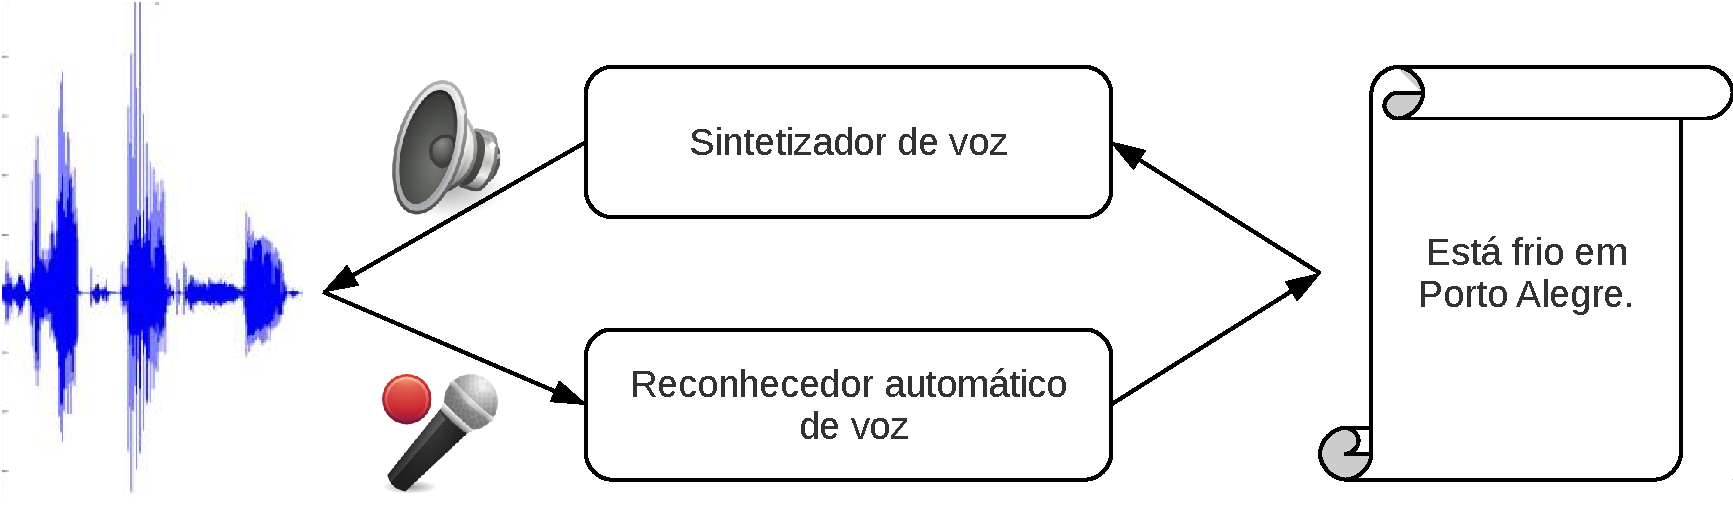
\includegraphics[height=3cm]{SintetizadorReconhecedor}
      \end{itemize}
   }

\begin{frame}
   \frametitle{Por que Reconhecimento Automático de Voz?}
   \vspace{0.5cm}
   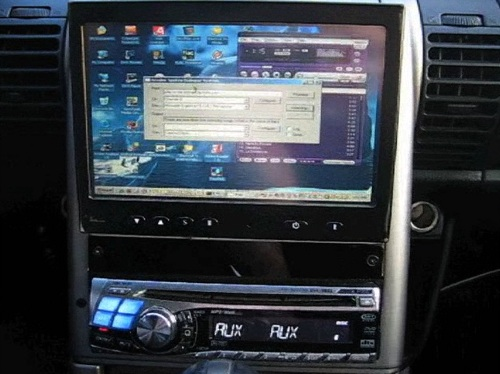
\includegraphics[height=3cm]{voice-controlled_car2}
   \hspace{1cm}
   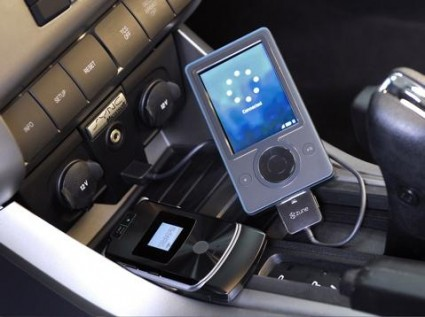
\includegraphics[height=3cm]{voice-controlled_car}\\

   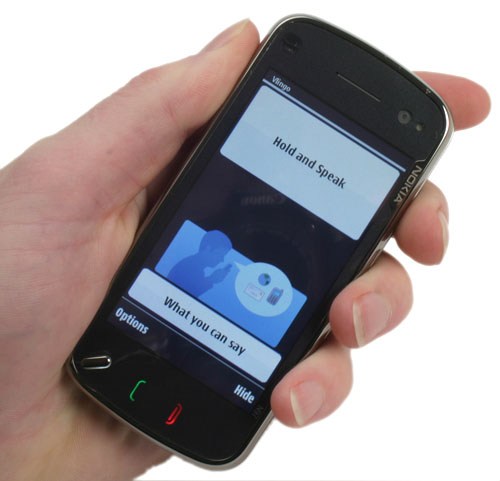
\includegraphics[height=3cm]{voice-controlled_phone}
   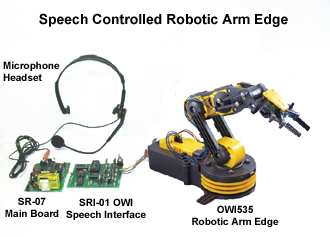
\includegraphics[height=4.5cm]{speech_controlled_robotic-arm}
\end{frame}

\section{A LaPSAPI}
\subsection{O que é a LaPSAPI?}
\frame{
   \frametitle{O Decodificador Julius e a LaPSAPI}
   \begin{itemize}
      \item Um importante integrante do RAV é o decodificador. Ele utiliza
	 os modelos acústicos e de linguagem para realizar a conversão dos
	 sinais de fala para texto.
      \begin{itemize}
	 \item Modos de operação:
	 \begin{itemize}
	    \item Comando e controle.
	    \item Ditado (ou fala espontânea).
	 \end{itemize}

	 \item Dependência de locutor.
	 \item Principais métricas de avaliação: precisão e velocidade.
      \end{itemize}

      \item É quem faz o reconhecimento propriamente dito.

      \item Para funcionar necessita de modelos acústico e de linguagem.

      \item LaPSAPI:
      \begin{itemize}
	 \item API de fácil uso.
	 \item Voltada para o desenvolvimento de
	    aplicações.

      \end{itemize}
   \end{itemize}
}

\subsection{O Uso da LaPSAPI}
\begin{frame}
   \frametitle{Como eu Posso Usar Essa API?}
   \begin{figure}
      \label{fig:interation_julius}
      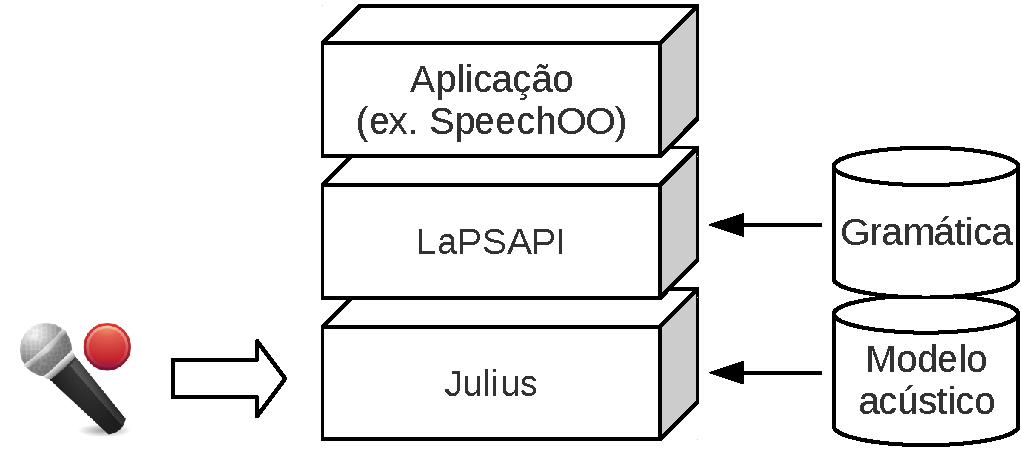
\includegraphics[height=1.5in]{API}
      \caption{Interação entre a aplicação do usuário, a LaPSAPI e o Julius}
   \end{figure}
\end{frame}

\begin{frame}[fragile]
   \frametitle{Informando para a Engine o que Reconhecer}
   \begin{itemize}
      \item Você deve definir uma gramática para informar a engine o
	 que ela deve esperar do usuário.

      \begin{figure}
	 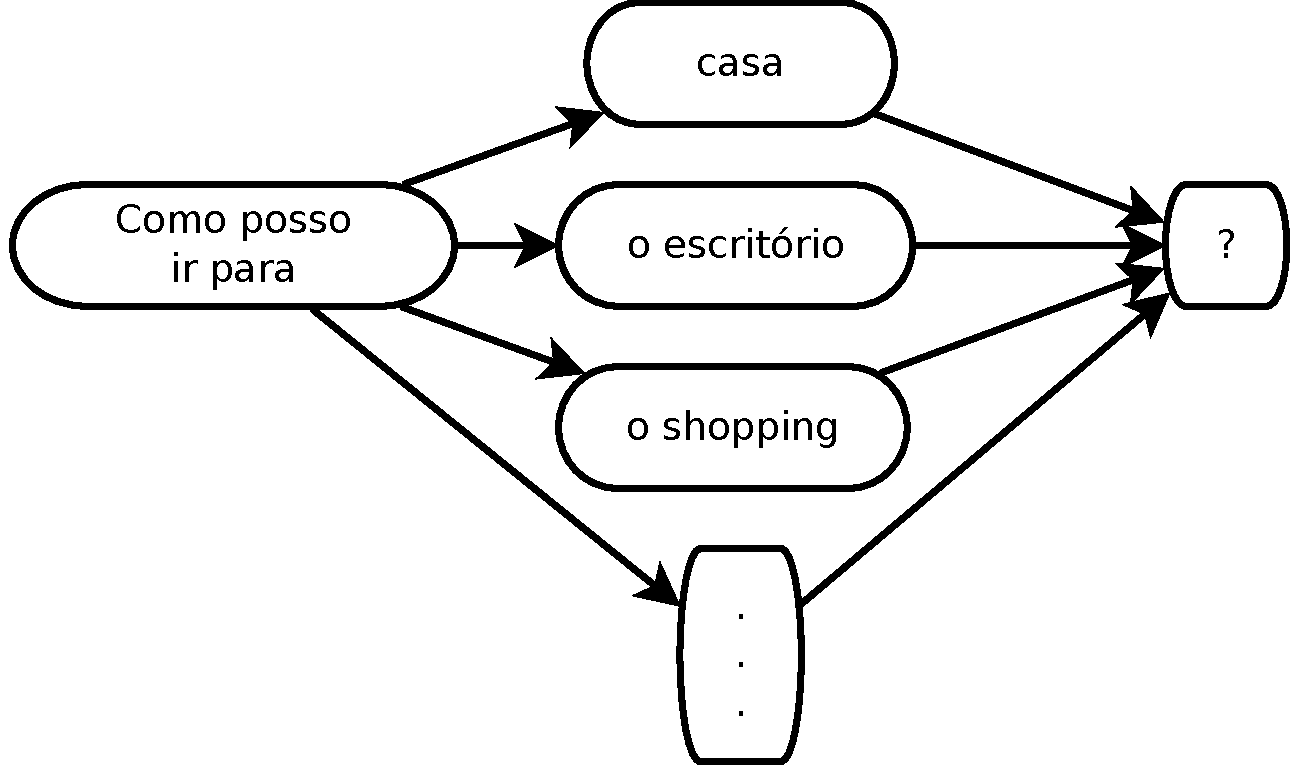
\includegraphics[height=1.5in]{grammar}
      \end{figure}

      \pause
      \item Você pode também usar modelo de língua para que
	 "tudo" possa ser reconhecido.
   \end{itemize}
\end{frame}

\section[Como Funciona?]{Como o Reconhecimento é Possível?}
\subsection{Definição}
\frame{
   \frametitle{Como Funciona Reconhecimento Automático de Voz?}
   \begin{itemize}
   \item A fala é uma sequencia de palavras.
      \item Cada palavra consiste em uma série de sons (fonemas).
      
      \item Dicionário fonético: conversão de uma sequência de caracteres
	 em sequência de fonemas.

      \item Modelos estatísticos baseados em probabilidades:
      \begin{itemize}
	 \item Acústica: cadeias escondidas de Markov (HMM).
	 \item Da língua: modelos n-gramas.
      \end{itemize}

      \item Modelos não-probabilisticos: gramáticas livre de contexto.
   \end{itemize}
}

\subsection{Os Modelos}
\begin{frame}
   \frametitle{O Conversor Grafema Fonema (G2P)}
   \begin{itemize}
      \item O dicionário fonético nos da a informação da correspondência
      entre a forma ortográfica e a pronuncia de uma palavra.\\
      {\centering \Large \texttt{noticia ->  n o tS i s i a}\\}
      \hspace{40pt} (grafema) \hspace{65pt} (fonema)\\[5pt]
   \end{itemize}
   \begin{itemize}
      \pause
      \item O LaPS disponibiliza um conversor G2P baseado em regras. Usamos
      este para gerar o dicionario fonético com 65 mil palavras.
   \end{itemize}
\end{frame}

\frame{
   \begin{center}
   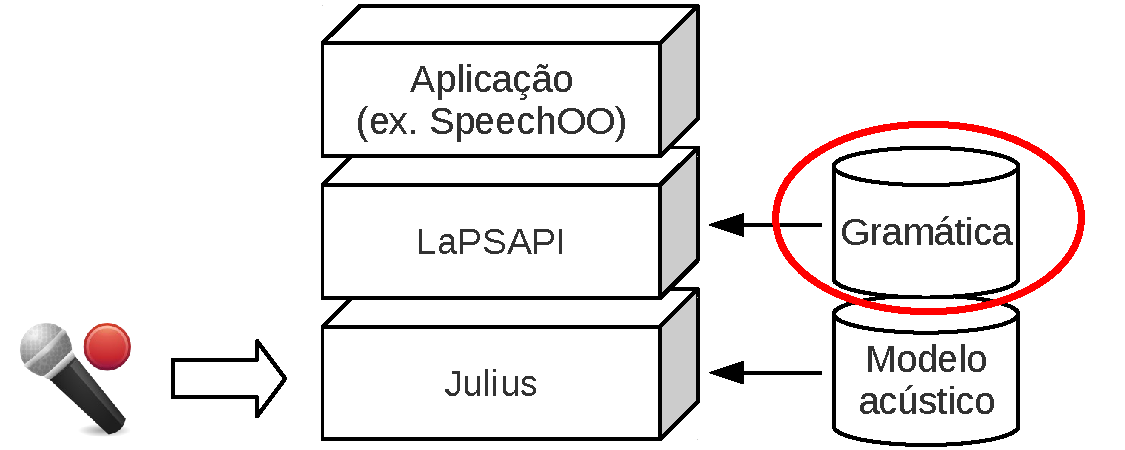
\includegraphics[height=1.5in]{API_grammar}
   \end{center}
}

\begin{frame}[fragile]
   \frametitle{O Corpora de Texto LaPSNews}
   \begin{itemize}
      \item O corpus de texto é simplesmente um conjunto de sentenças.
      {\footnotesize
	 \begin{verbatim}
<s> a cidade não vai se livrar do minhocão </s>
<s> segundo a escola os dois casos não têm relação </s>
<s> meu filho estava a poucos metros de casa </s>
...
	    \end{verbatim}
      }
      \pause
      \item LaPSNews:
      \begin{itemize}
	 \item Baseado na coleta diária de textos da internet (crawling).
	 \item Foram coletadas mais de 1 milhão de sentenças.
      \end{itemize}
   \end{itemize}
\end{frame}

\frame{
   \begin{center}
   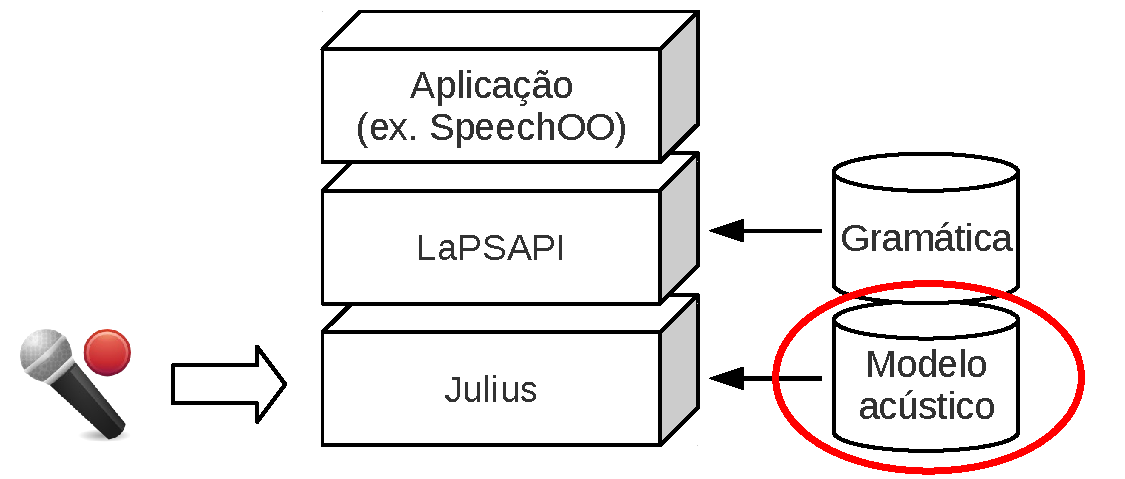
\includegraphics[height=1.5in]{API_am}
   \end{center}
}

\begin{frame}
   \frametitle{Corpora de Áudio}
   \begin{itemize}
      \item Para obter um AM robusto necessita-se de uma grande
      quantidade de áudio transcrito.
      \item Para Português brasileiro nos temos certa de 20 horas
      de áudio de boa qualidade transcrito.
      \item Outras línguas como o Inglês tem corpus com mais de 240 horas.
      \begin{center}
	 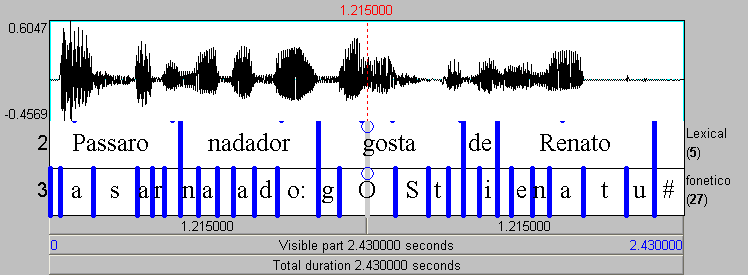
\includegraphics[height=1.5in]{sound_transcription}
      \end{center}
   \end{itemize}
\end{frame}

\subsection{O Sistema}
\frame{
   \frametitle{Processo de Reconhecimento}
   \begin{center}
      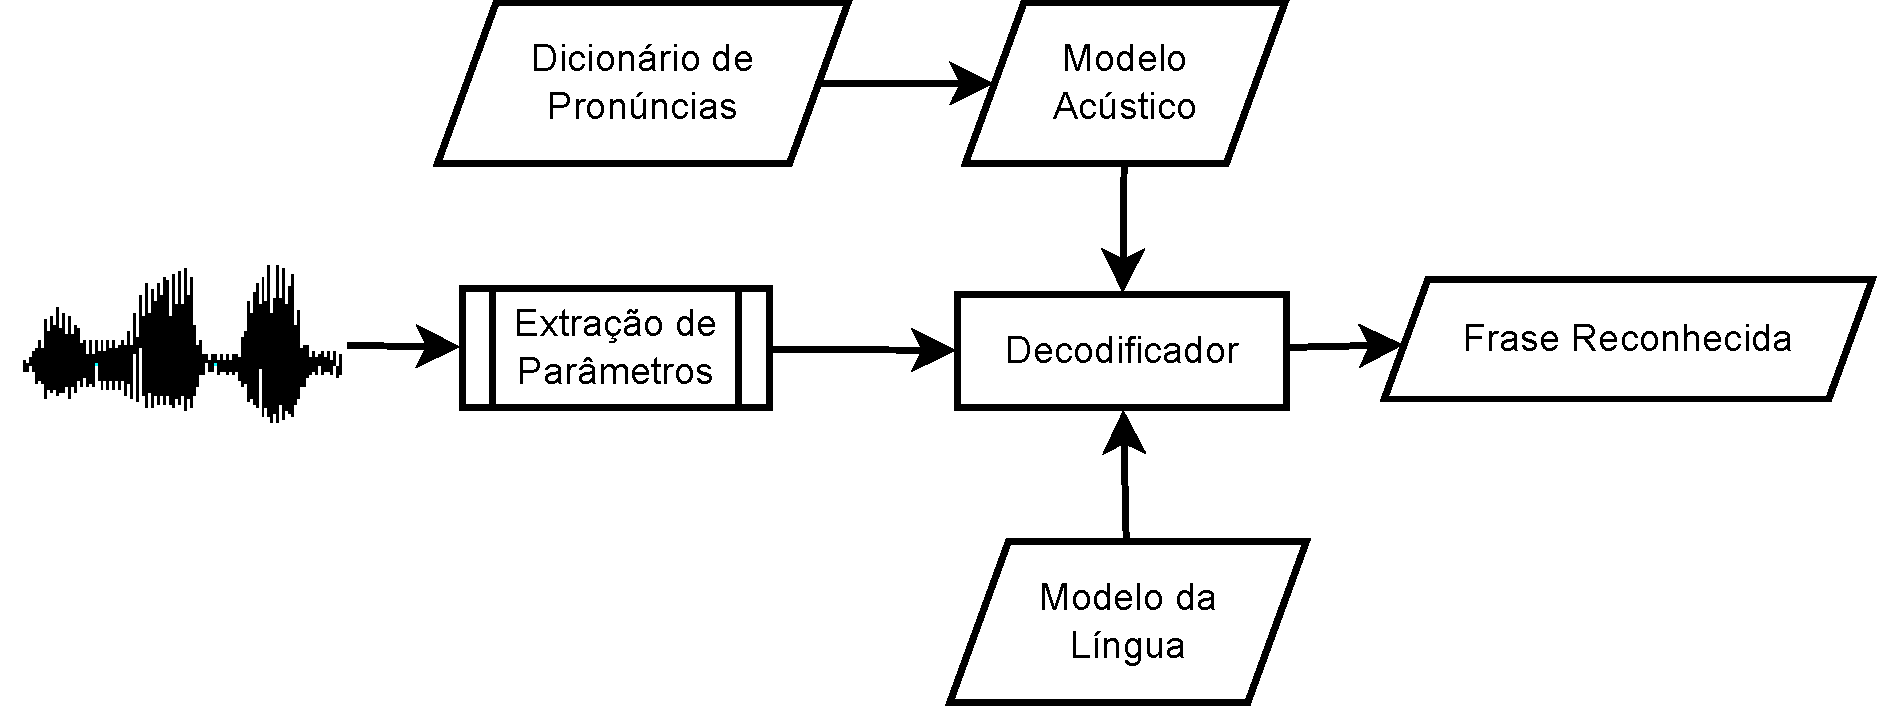
\includegraphics[height=1.4in]{diagrama_reconhecimento}
   \end{center}
}

\section{Desempenho}
\subsection[Comparação]{Comparação entre HDecode, IBM ViaVoice e Julius}
\begin{frame}
   \frametitle{Quão Bom é o Reconhecedor?}
   \begin{itemize}
      \item Três software (modelos) foram avaliados.
      \begin{itemize}
	 \item HDecode.
	 \item Julius.
	 \item Software comercial (IBM ViaVoice).
      \end{itemize}

      \item Medidas de performance.
      \begin{itemize}
	 \item WER (word error rate).
	 \item xRT (real-time factor).
      \end{itemize}

      \item A avaliação foi dividida em duas etapas:
      \begin{itemize}
	 \item Modelo dependente de locutor.
	 \item Modelo independente de locutor.
      \end{itemize}
   \end{itemize}
\end{frame}

\begin{frame}
   \frametitle{Comparação usando Modelos Independentes de Locutor}
   \begin{itemize}
      \item Os modelos LaPSAM e LaPSLM foram usados com Julius e HDecode.
      \begin{table}
	 \centering
	 \begin{tabular}{ l c c }
	    \toprule
	    \textbf{Decoder} & \textbf{WER(\%)} & \textbf{xRT} \\\midrule
	    Julius & 29 & 0.99 \\\midrule
	    HDecode & 20.13 & 1.2 \\\midrule
	    IBM ViaVoice & 29.30 & - \\
	     \bottomrule
	  \end{tabular}
	  \caption{Comparação dos sistemas usando modelos independentes de locutor.}
       \end{table}
    \end{itemize}
\end{frame}

\begin{frame}
   \frametitle{Comparação usando Modelos Dependentes de Locutor}
   \begin{itemize}
      \item Dois modelos dependentes de locutor foram comparados.
      \item Para cada adaptação foram usados 10 minutos de áudio.
      \begin{center}
      \begin{table}
	 \begin{tabular}{ l c c }
	    \toprule
	    \textbf{Decoder} & \textbf{CWR(\%)} & \textbf{xRT} \\\midrule
	    Julius & 13.30 & 0.99 \\\midrule
	    HDecode & 6.81 & 0.91 \\\midrule
	    IBM ViaVoice & 17.30 & - \\
	    \bottomrule
	 \end{tabular}
	 \caption{Comparação dos sistemas usando modelos dependentes de locutor.}
      \end{table}
      \end{center}
   \end{itemize}
\end{frame}


\section{Considerações Finais}
\subsection{Aplicativos Desenvolvidos}
\frame{
   \frametitle{CorujaNavigator: Um Navegador Web não visual e hands-free}
   \begin{itemize}
      \item Navegação web exclusivamente através de texto.
      \begin{itemize}
	 \item O usuário diz da página atual que quer acessar.
	 \item O CorujaNavigator acessa e sintetiza o texto da nova página.
      \end{itemize}
      \item Atualmente necessita de métodos para cada domínio a ser acessado.
      \begin{itemize}
	 \item Estamos trabalhando para que o acesso seja livre de domínio.
      \end{itemize}
   \end{itemize}
}

\frame{
   \frametitle{SpeechOO: Ditado no OpenOffice.org}
   \begin{itemize}
      \item Faz uso do pacote Coruja para permitir ditado
	 para o aplicativo Writer do OpenOffice.org.
      \begin{itemize}
	 \item Permite apenas o ditado.
      \end{itemize}

      \pause
      \item Trabalhos Futuros:
      \begin{itemize}
	 \item Possibilitar comandos, como: Negrito, tamanho da fonte, etc.
	 \item Passar a sentença pelo corretor gramatical para corrigir
	    possíveis erros.
	 \item Módulo para fazer recase da sentença reconhecida.
	 \item Permitir a correção de uma palavra que foi reconhecida errado.
	 \item Acrescentar módulo de adaptação de locutor (aguardando módulo do
	       Coruja).
      \end{itemize}
   \end{itemize}
}

\frame{
   \frametitle{Arquitetura do SpeechOO}
   \begin{center}
   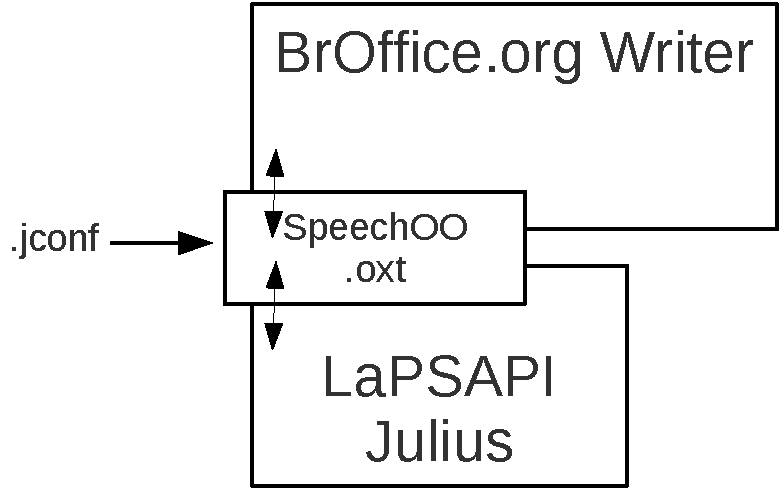
\includegraphics[height=2.5in]{arq_speechoo}
   \end{center}
}


\subsection{Trabalhos Públicados e Palestras}
\frame{
\begin{itemize}
{\footnotesize
\item Patrick Silva, Pedro Batista, Nelson Neto, Aldebaro Klautau. \textit{An Open-Source
Speech Recognizer for Brazilian Portuguese with a Windows Programming
Interface.}
Em: The International Conference on Computational Processing of the Portuguese Language -
PROPOR 2010, Porto Alegre.\\

\item Pedro Batista, Patrick Silva, Nelson Neto, Aldebaro Klautau.
\textit{A non-Visual Web Browsing System using Speech Recognition for Brazilian Portuguese}
Em: The International Conference on Computational Processing of the Portuguese Language -
Demos Session PROPOR 2010, Porto Alegre.\\

\item Pedro Batista, William Colem. \textit{"Veja mamãe,
sem as mãos!" SpeechOO, uma extensão de ditado para o BrOffice.org}
Em: Palestra no concorrido Fórum Internacional de Software Livre - FISL 11, Porto Alegre 2010.\\

\item O \textit{software} Coruja Navigator recebeu o prêmio: \textit{Melhor Produto
de Software do Pará na Categoria Acadêmico}. Premiação concedida pelo Laboratório de Tecnologia
de Software da UFPA no IX Simpósio Brasileiro de Qualidade de Software.\\

\item Pedro Batista. \textit{Desenvolvimento de Aplicativos Utilizando Reconhecimento Automático de Voz
Para Português Brasileiro} Em: Palestra na Semana Acadêmica do CBCC.\\
}
\end{itemize}
}

\begin{frame}
   \large
   \frametitle{Obrigado! Perguntas?}
   \begin{figure}
      
\includegraphics[height=1in]{logo}\\
      
\includegraphics[height=0.8in]{logo_ufpa}
      
\includegraphics[height=0.4in]{logo_laps}\\
      
\includegraphics[height=1.1in]{logo_cnpq}
      
\includegraphics[height=0.7in]{logo_fapespa}
   \end{figure}
\end{frame}

\end{document}
